\documentclass[../main.tex]{subfiles}
\graphicspath{{\subfix{../Images/}}}

\begin{document}

\chapter{Chapter 5. Lighting}

This chapter shows you how to illuminate the objects in your scenes with light sources. We start by building a simplified version of a commonly used lighting model. Then, we gradually add functionality to the basic model to make it more useful in common situations. This chapter has the following five sections:

\begin{itemize}
\item \textbf{"Lighting and Lighting Models"} explains the importance of lighting and introduces the concept of a lighting model.
\item \textbf{"Implementing the Basic Per-Vertex Lighting Model"} presents a simplified version of the lighting model used in OpenGL and Direct3D. This section also goes through a step-by-step implementation of this lighting model in a vertex program.
\item \textbf{"Per-Fragment Lighting"} describes the differences between per-vertex and per-fragment lighting and shows you how to implement per-fragment lighting.
\item \textbf{"Creating a Lighting Function"} explains how to create your own functions.
\item \textbf{"Extending the Basic Model"} describes several improvements to the basic lighting model, including texturing, attenuation, and spotlight effects. While explaining these improvements, we introduce several key Cg concepts, such as creating functions, arrays, and structures.
\end{itemize}

\section{5.1 Lighting and Lighting Models}

So far, all our examples have been straightforward, focusing on the fundamental concepts that you need to start writing programs. The next few chapters will show you how to add some more interesting effects. This chapter explains lighting.

Adding a light to a scene causes many variations in shading and creates more interesting images. This is why movie directors pay such close attention to lighting: it plays a big part in telling a compelling story. Dark areas of a scene can evoke a sense of mystery and heightened tension. (Unfortunately, in computer graphics, shadows do not come "for free" when you add lights to a scene. Chapter 9 visits the separate topic of shadow generation.)

Together, lighting and an object's material properties determine its appearance. A lighting model describes the way light interacts with an object, based on the light's characteristics and the object material's characteristics. Over the years, numerous lighting models have been developed and used, ranging from simple approximations to extremely accurate simulations.

Figure \ref{fig:5-1} shows a set of objects that were rendered using various lighting models. Notice how the different formulations resemble an assortment of real-world materials.

\begin{figure}
    \centering
    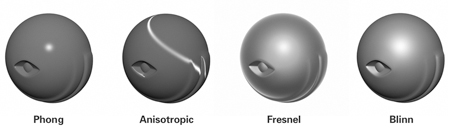
\includegraphics[width=1\linewidth]{fig5_1.jpg}
    \caption{Figure 5-1 Different Lighting Models}
    \label{fig:5-1}
\end{figure}

In the past, fixed-function graphics pipelines were limited to one lighting model, which we call the \textit{fixed-function lighting model}. The fixed-function model is based on what is known as the Phong lighting model, but with some tweaks and additions. The fixed-function lighting model has several advantages: it looks adequate, it's cheap to compute, and it has a number of intuitive parameters that can be tweaked to control appearance. The problem with it, however, is that it works well for only a limited set of materials. A plastic or rubbery appearance is the most common symptom of using the fixed-function lighting model, and this explains why many computer graphics images do not look realistic.

To get around the limitations of the fixed-function lighting model, graphics programmers found innovative ways to use other features of the pipeline. For example, clever programs used texture-based methods to mimic the surface characteristics of a wider range of materials.

With the advent of Cg and programmable hardware, you can now express complicated lighting models concisely using a high-level language. You no longer have to configure a limited set of graphics pipeline states or program tedious assembly language routines. And, you don't have to limit your lighting model to fit the fixed-function pipeline's capabilities. Instead, you can express your own custom lighting model as a Cg program that executes within your programmable GPU.

\section{5.2 Implementing the Basic Per-Vertex Lighting Model}

This section explains how to implement a simplified version of the fixed-function lighting model using a vertex program. The familiarity and simplicity of this lighting model make it an excellent starting point. First we give some background about the fixed-function lighting model. If you are already familiar with this lighting model, feel free to skip ahead to the implementation in Section 5.2.2.

\subsection{5.2.1 The Basic Lighting Model}

OpenGL and Direct3D provide almost identical fixed-function lighting models. In our example, we will use a simplified version that we will refer to as the "Basic" model. The Basic model, like the OpenGL and Direct3D models, modifies and extends the classic Phong model. In the Basic model, an object's surface color is the sum of emissive, ambient, diffuse, and specular lighting contributions. Each contribution depends on the combination of the surface's material properties (such as shininess and material color) and the light source's properties (such as light color and position). We represent each contribution as a \textbf{float3} vector that contains the red, green, and blue color components.

This high-level equation describes the Basic model mathematically:

$surfaceColor = emissive + ambient + diffuse + specular$

\subsection*{The Emissive Term}

The emissive term represents light emitted or given off by a surface. This contribution is independent of all light sources. The emissive term is an RGB value that indicates the color of the emitted light. If you were to view an emissive material in a completely dark room, it would appear to be this color. The emissive term can simulate glowing. Figure \ref{fig:5-2} illustrates the emissive term conceptually, and Figure \ref{fig:5-3} shows a rendering of a purely emissive object. The rendering is understandably boring, because the emissive color is the same all over the object. Unlike in the real world, an object's emissive glow does not actually illuminate other nearby objects in the scene. An emissive object is not itself a light source—it does not illuminate other objects or cast shadows. Another way to think of the emissive term is that it is a color added after computing all the other lighting terms. More advanced global illumination models would simulate how the emitted light affects the rest of the scene, but these models are beyond the scope of this book.

\begin{figure}
    \centering
    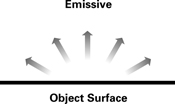
\includegraphics[width=0.5\linewidth]{fig5_2.jpg}
    \caption{Figure 5-2 The Emissive Term}
    \label{fig:5-2}
\end{figure}

\begin{figure}
    \centering
    
\includegraphics[width=0.5\linewidth]{fig5_3.jpg}
    \caption{Figure 5-3 Rendering the Emissive Term}
    \label{fig:5-3}
\end{figure}

Here is the mathematical formulation we use for the emissive term:

$emissive = K_e$

where:

\begin{itemize}
    \item \textit{K\textsubscript{e}} is the material's emissive color.
\end{itemize}

\subsection*{The Ambient Term}

The ambient term accounts for light that has bounced around so much in the scene that it seems to come from everywhere. Ambient light does not appear to come from any particular direction; rather, it appears to come from all directions. Because of this, the ambient lighting term does not depend on the light source position. Figure \ref{fig:5-4} illustrates this concept, and Figure \ref{fig:5-5} shows a rendering of an object that receives only ambient light. The ambient term depends on a material's ambient reflectance, as well as the color of the ambient light that is incident on the material. Like the emissive term, the ambient term on its own is just a constant color. Unlike the emissive color, however, the ambient term is affected by the global ambient lighting.

\begin{figure}
    \centering
    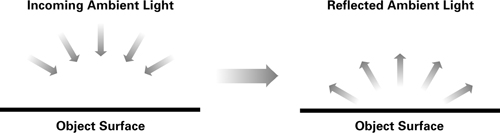
\includegraphics[width=1\linewidth]{fig5_4.jpg}
    \caption{Figure 5-4 The Ambient Term}
    \label{fig:5-4}
\end{figure}

\begin{figure}
    \centering
    
\includegraphics[width=0.5\linewidth]{fig5_5.jpg}
    \caption{Figure 5-5 Rendering the Ambient Term}
    \label{fig:5-5}
\end{figure}

Here is the mathematical formulation we use for the ambient term:

$ambient = K_a * globalAmbient$

where:

\begin{itemize}
\item \textit{K\textsubscript{a}} is the material's ambient reflectance and
\item \textit{globalAmbient} is the color of the incoming ambient light.
\end{itemize}

\subsection*{The Diffuse Term}

The diffuse term accounts for directed light reflected off a surface equally in all directions. In general, diffuse surfaces are rough on a microscopic scale, with small nooks and crannies that reflect light in many directions. When incoming rays of light hit these nooks and crannies, the light bounces off in all directions, as shown in Figure \ref{fig:5-6}.

\begin{figure}
    \centering
    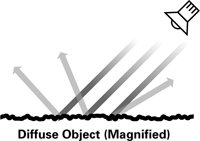
\includegraphics[width=0.5\linewidth]{fig5_6.jpg}
    \caption{Figure 5-6 Diffuse Light Scattering}
    \label{fig:5-6}
\end{figure}

The amount of light reflected is proportional to the angle of incidence of the light striking the surface. Surfaces with a dull finish, such as a dusty chalkboard, are said to be diffuse. The diffuse contribution at any particular point on a surface is the same, regardless of where the viewpoint is. Figure \ref{fig:5-7} illustrates the diffuse term, and Figure \ref{fig:5-8} shows a rendering of a diffuse object.

\begin{figure}
    \centering
    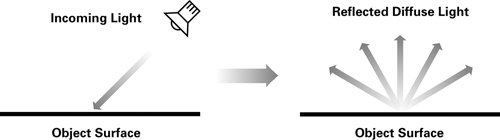
\includegraphics[width=1\linewidth]{fig5_7.jpg}
    \caption{Figure 5-7 The Diffuse Term}
    \label{fig:5-7}
\end{figure}

\begin{figure}
    \centering
    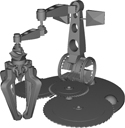
\includegraphics[width=0.5\linewidth]{fig5_8.jpg}
    \caption{Figure 5-8 Rendering the Diffuse Term}
    \label{fig:5-8}
\end{figure}

Here is the mathematical formulation we use for the diffuse term (illustrated in Figure \ref{fig:5-9}):

$diffuse = K_d * lightColor * max(N \cdot L, 0)$

where:

\begin{itemize}
\item \textit{K\textsubscript{d}} is the material's diffuse color,
\item \textit{lightColor} is the color of the incoming diffuse light,
\item \textit{N} is the normalized surface normal,
\item \textit{L} is the normalized vector toward the light source, and
\item \textit{P} is the point being shaded.
\end{itemize}

\begin{figure}
    \centering
    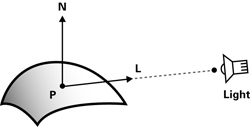
\includegraphics[width=0.75\linewidth]{fig5_9.jpg}
    \caption{Figure 5-9 Calculating Diffuse Lighting}
    \label{fig:5-9}
\end{figure}

The vector dot product (or inner product) of the normalized vectors \textit{N} and \textit{L} is a measure of the angle between the two vectors. The smaller the angle between the vectors, the greater the dot-product value will be, and the more incident light the surface will receive. Surfaces that face away from the light will produce negative dot-product values, so the $max(N \cdot L, 0)$ in the equation ensures that these surfaces show no diffuse lighting.

\subsection*{The Specular Term}

The specular term represents light scattered from a surface predominantly around the mirror direction. The specular term is most prominent on very smooth and shiny surfaces, such as polished metals. Figure \ref{fig:5-10} illustrates the concept of specular reflection, and Figure \ref{fig:5-11} shows a rendering of a completely specular object.

\begin{figure}
    \centering
    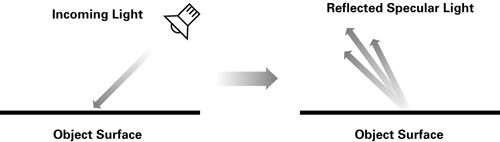
\includegraphics[width=1\linewidth]{fig5_10.jpg}
    \caption{Figure 5-10 The Specular Term}
    \label{fig:5-10}
\end{figure}

\begin{figure}
    \centering
    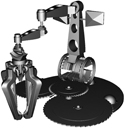
\includegraphics[width=0.5\linewidth]{fig5_11.jpg}
    \caption{Figure 5-11 Rendering the Specular Term}
    \label{fig:5-11}
\end{figure}

Unlike the emissive, ambient, and diffuse lighting terms, the specular contribution depends on the location of the viewer. If the viewer is not at a location that receives the reflected rays, the viewer will not see a specular highlight on the surface. The specular term is affected not only by the specular color properties of the light source and material, but also by how shiny the surface is. Shinier materials have smaller, tighter highlights, whereas less shiny materials have highlights that are more spread out. Figure \ref{fig:5-12} shows some examples of shininess, with the shininess exponent increasing from left to right.

\begin{figure}
    \centering
    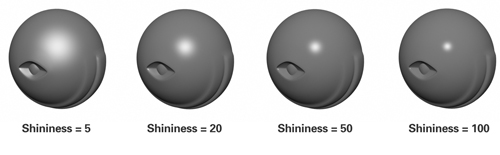
\includegraphics[width=1\linewidth]{fig5_12.jpg}
    \caption{Figure 5-12 Examples of Different Shininess Exponents}
    \label{fig:5-12}
\end{figure}

Here is the mathematical formulation we use for the specular term (illustrated in Figure \ref{fig:5-13}):

$specular = K_s * lightColor * facing * (max(N \cdot H, 0)) ^{shininess}$

where:

\begin{itemize}
\item \textit{K\textsubscript{s}} is the material's specular color,
\item \textit{lightColor} is the color of the incoming specular light,
\item \textit{N} is the normalized surface normal,
\item \textit{V} is the normalized vector toward the viewpoint,
\item \textit{L} is the normalized vector toward the light source,
\item \textit{H} is the normalized vector that is halfway between \textit{V} and \textit{L},
\item \textit{P} is the point being shaded, and
\item \textit{facing} is 1 if $N \cdot L$ is greater than 0, and 0 otherwise.
\end{itemize}

\begin{figure}
    \centering
    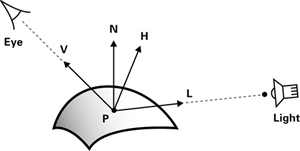
\includegraphics[width=0.75\linewidth]{fig5_13.jpg}
    \caption{Figure 5-13 Calculating the Specular Term}
    \label{fig:5-13}
\end{figure}

When the angle between the view vector \textit{V} and the half-angle vector \textit{H} is small, the specular appearance of the material becomes apparent. The exponentiation of the dot product of \textit{N} and \textit{H} ensures that the specular appearance falls off quickly as \textit{H} and \textit{V} move farther apart.

Additionally, the specular term is forced to zero if the diffuse term is zero because $N \cdot L$ (from diffuse lighting) is negative. This ensures that specular highlights do not appear on geometry that faces away from the light.

\subsection*{Adding the Terms Together}

Combining the ambient, diffuse, and specular terms gives the final lighting, as shown in Figure \ref{fig:5-14}. In the figure, we deliberately exclude the emissive term, because it is normally used to achieve special effects rather than for lighting ordinary objects.

\begin{figure}
    \centering
    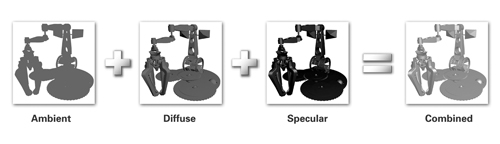
\includegraphics[width=1\linewidth]{fig5_14.jpg}
    \caption{Figure 5-14 Putting the Terms Together}
    \label{fig:5-14}
\end{figure}

\subsection*{Simplifications}

If you are experienced with OpenGL or Direct3D, you might have noticed a number of simplifications for the Basic lighting model. We are using a global ambient color instead of a per-light ambient color. We are also using the same value for the light's diffuse and specular colors instead of allowing different values for each of these. In addition, we do not account for attenuation or spotlight effects.

\subsection{5.2.2 A Vertex Program for Basic Per-Vertex Lighting}

This section explains a Cg vertex program that implements the Basic lighting model described in Section 5.2.1

The \textbf{C5E1v_basicLight} vertex program in Example 5-1 does the following:

\begin{enumerate}
\item Transforms the position from object space to clip space.
\item Computes the illuminated color of the vertex, including the emissive, ambient, diffuse, and specular lighting contributions from a single light source.
\end{enumerate}

In this example, we perform the lighting calculations in object space. You could also use other spaces, provided that you transform all necessary vectors into the appropriate coordinate system. For example, OpenGL and Direct3D perform their lighting computations in eye space rather than object space. Eye space is more efficient than object space when there are multiple lights, but object space is easier to implement.

\FloatBarrier
\begin{lstlisting}[caption=Example 5-1. The C5E1v_basicLight Vertex Program]
void C5E1v_basicLight(float4 position  : POSITION,
                      float3 normal    : NORMAL,

                  out float4 oPosition : POSITION,
                  out float4 color     : COLOR,

              uniform float4x4 modelViewProj,
              uniform float3 globalAmbient,
              uniform float3 lightColor,
              uniform float3 lightPosition,
              uniform float3 eyePosition,
              uniform float3 Ke,
              uniform float3 Ka,
              uniform float3 Kd,
              uniform float3 Ks,
              uniform float  shininess)
{
  oPosition = mul(modelViewProj, position);

  float3 P = position.xyz;
  float3 N = normal;

  // Compute the emissive term
  float3 emissive = Ke;

  // Compute the ambient term
  float3 ambient = Ka * globalAmbient;

  // Compute the diffuse term
  float3 L = normalize(lightPosition - P);
  float diffuseLight = max(dot(N, L), 0);
  float3 diffuse = Kd * lightColor * diffuseLight;

  // Compute the specular term
  float3 V = normalize(eyePosition - P);
  float3 H = normalize(L + V);
  float specularLight = pow(max(dot(N, H), 0),
                            shininess);
  if (diffuseLight <= 0) specularLight = 0;
  float3 specular = Ks * lightColor * specularLight;

  color.xyz = emissive + ambient + diffuse + specular;
  color.w = 1;
}
\end{lstlisting}
\FloatBarrier

The exercises at the end of this chapter explore the trade-offs between eye-space and object-space lighting.

\subsection*{Application-Specified Data}

Table \ref{table:5-1} lists the various pieces of data that the application needs to send to the graphics pipeline. We classify each item as \textit{varying} if the item changes with every vertex, or \textit{uniform} if the item changes less frequently (such as on a per-object basis).

\begin{table}
\centering
\begin{tabular}{ p{5cm} p{5cm} p{2cm} p{2cm}  } 

Parameter & Variable Name & Type & Category \\
\hline

\multicolumn{4}{p{10cm}}{\textbf{GEOMETRIC PARAMETERS}}\\
	 	 
Object-space vertex position & \textbf{position} & \textbf{float4} & Varying \\
Object-space vertex normal & \textbf{normal} & \textbf{float3} & Varying \\
Concatenated modelview and projection matrices & \textbf{modelViewProj} & \textbf{float4x4} & Uniform \\
Object-space light position & \textbf{lightPosition} & \textbf{float3} & Uniform \\
Object-space eye position & \textbf{eyePosition} & \textbf{float3} & Uniform \\

\hline

\multicolumn{4}{p{10cm}}{\textbf{LIGHT PARAMETERS}}\\
Light color & \textbf{lightColor} & \textbf{float3} & Uniform \\
Global ambient color & \textbf{globalAmbient} & \textbf{float3} & Uniform \\

\hline

\multicolumn{4}{p{10cm}}{\textbf{MATERIAL PARAMETERS}}\\
Emissive reflectance & \textbf{K\textsubscript{e}} & \textbf{float3} & Uniform \\
Ambient reflectance & \textbf{K\textsubscript{a}} & \textbf{float3} & Uniform \\
Diffuse reflectance & \textbf{K\textsubscript{d}} & \textbf{float3} & Uniform \\
Specular reflectance & \textbf{K\textsubscript{s}} & \textbf{float3} & Uniform \\
Shininess & \textbf{shininess} & \textbf{float} & Uniform \\
\hline

\end{tabular}

\caption{Table 5-1. Application-Specified Data for the Graphics Pipeline}
\label{table:5-1}
\end{table}

\subsection*{A Debugging Tip}

As you can see, the code for lighting is significantly more complex than any Cg code you have seen so far. When you are working on a program that is not trivial, it is a good idea to build it up slowly, piece by piece. Run the program as you make each incremental addition, and check to make sure that the results are what you expect. This is much smarter than writing all the code for the program and then hoping that it generates the right result. If you make a minor error, tracking down a problem will be a lot easier if you know the recent changes that probably caused it.

This tip applies particularly to lighting code, because lighting can be broken down into various contributions (emissive, ambient, diffuse, and specular). Therefore, a good approach is to calculate \textbf{emissive}, and then set color to just \textbf{emissive}. After that, calculate \textbf{ambient}, and set \textbf{color} to \textbf{emissive} plus \textbf{ambient}. By building up your Cg programs gradually in this manner, you will save yourself a lot of frustration.

\subsection*{The Vertex Program Body}

\subsection*{\textit{Calculating the Clip-Space Position}}

We start by computing the usual clip-space position calculation for the rasterizer, as explained in Chapter 4:
\FloatBarrier
\begin{lstlisting}
   oPosition = mul(modelViewProj, position);
\end{lstlisting}
\FloatBarrier

Next, we instance a variable to store the object-space vertex position, because we will need this information later on. We are going to use a \textbf{float3} temporary variable because the other vectors used in lighting (such as the surface normal, light position, and eye position) are also \textbf{float3} types.

\FloatBarrier
\begin{lstlisting}
float3 P = position.xyz;
\end{lstlisting}
\FloatBarrier

Here we see an interesting new piece of syntax: \textbf{position.xyz} . This is our first look at a feature of Cg called \textit{swizzling}.

By ignoring the object-space \textit{w} component, we are effectively assuming that \textit{w} is 1.

\subsection*{\textit{Swizzling}}

Swizzling allows you to rearrange the components of a vector to create a new vector—in any way that you choose. Swizzling uses the same period operator that is used to access structure members, plus a suffix that indicates how you would like to rearrange the components of a vector that you're working on. The suffix is some combination of the letters \textbf{x}, \textbf{y}, \textbf{z}, and \textbf{w}. The letters \textbf{r}, \textbf{g}, \textbf{b}, and \textbf{a} —appropriate for RGBA colors—can also be used. However, the two sets of suffix letters cannot be mixed. These letters indicate which components of the original vector to use when constructing the new one. The letters \textbf{x} and \textbf{r} correspond to the first component of a vector, \textbf{y} and \textbf{g} to the second component, and so on. In the previous example, \textbf{position} is a \textbf{float4} variable. The \textbf{.xyz} suffix extracts the \textit{x}, \textit{y}, and \textit{z} components of \textbf{position} and creates a new three-component vector from these three values. This new vector is then assigned to the \textbf{float3} variable called \textbf{P}.

Neither C nor C++ supports swizzling because neither language has built-in support for vector data types. However, swizzling is quite useful in Cg to manipulate vectors efficiently.

Here are some more examples of swizzling:

\FloatBarrier
\begin{lstlisting}
float4 vec1 = float4(4.0, -2.0, 5.0, 3.0);
float2 vec2 = vec1.yx;        // vec2 = (-2.0, 4.0)
float scalar = vec1.w;        // scalar = 3.0
float3 vec3 = scalar.xxx;     // vec3 = (3.0, 3.0, 3.0)
\end{lstlisting}
\FloatBarrier

Take a closer look at these four lines of code. The first line declares a \textbf{float4} called \textbf{vec1}. The second line takes the \textbf{y} and \textbf{x} components of \textbf{vec1} and creates a swapped \textbf{float2} out of them. This vector is then assigned to \textbf{vec2}. In the third line, the \textbf{w} component of \textbf{vec1} is assigned to a single \textbf{float}, called \textbf{scalar}. Finally, in the last line, a \textbf{float3} vector is created by replicating \textbf{scalar} three times. This is known as \textit{smearing}, and it illustrates that Cg treats scalar values just like one component vector (meaning that the \textbf{.x} suffix is used to access the scalar's value).

You can also swizzle matrices to create vectors based on a sequence of matrix elements. To do this, use the \textbf{._m <row><col>} notation. You can chain together a series of matrix swizzles, and the result will be an appropriately sized vector. For example:

\FloatBarrier
\begin{lstlisting}
float4x4 myMatrix;
float    myFloatScalar;
float4   myFloatVec4;'

// Set myFloatScalar to myMatrix[3][2]
myFloatScalar = myMatrix._m32;

// Assign the main diagonal of myMatrix to myFloatVec4
myFloatVec4 = myMatrix._m00_m11_m22_m33;
\end{lstlisting}
\FloatBarrier

In addition, you can access an individual row of a matrix using the \textbf{[}] array operator. Using the variables declared in the preceding code sample:

\FloatBarrier
\begin{lstlisting}
// Set myFloatVector to the first row of myMatrix
myFloatVec4 = myMatrix[0];
\end{lstlisting}
\FloatBarrier

\subsection*{\textit{Write Masking}}

Cg supports another operation, related to swizzling, called \textit{write masking}, that allows only specified components of a vector to be updated by an assignment. For example, you could write to just the \textit{x} and \textit{w} components of a \textbf{float4} vector by using a \textbf{float2} vector:

\FloatBarrier
\begin{lstlisting}
// Assume that initially vec1 = (4.0, -2.0, 5.0, 3.0)
//                   and vec2 = (-2.0, 4.0);
vec1.xw = vec2;  // Now vec1 = (-2.0, -2.0, 5.0, 4.0)
\end{lstlisting}
\FloatBarrier

The write-masking suffix can list the \textbf{x}, \textbf{y}, \textbf{z}, and \textbf{w} (or \textbf{r}, \textbf{g}, \textbf{b}, and \textbf{a}) components in any order. Each letter can appear at most once in a given write-mask suffix, and you cannot mix the \textbf{xyzw} and \textbf{rgba} letters in a single write-mask suffix.

\begin{framed}
Performance Tip

On most modern GPUs, swizzling and write masking are operations that have no performance penalty. So use both features whenever they help improve the clarity or efficiency of your code.
\end{framed}

\subsection*{\textit{The Emissive Light Contribution}}

There is nothing much to do for the emissive term. For the sake of coding clarity, we instance a variable, named \textbf{emissive}, for the emissive light contribution:

\FloatBarrier
\begin{lstlisting}
   // Compute emissive term
   float3 emissive = Ke;
\end{lstlisting}
\FloatBarrier

\begin{framed}
Coding Tip

When the Cg compiler translates your program to executable code, it also optimizes the translated code so that there is no performance penalty for creating intermediate variables such as the \textbf{emissive} variable in the above code fragment. Because instancing such variables makes your code more readable, you are encouraged to instance named variables for intermediate results to improve the clarity of your code.
\end{framed}

\subsection*{\textit{The Ambient Light Contribution}}

For the ambient term, recall that we have to take the material's ambient color, \textbf{Ka}, and multiply it by the global ambient light color. This is a per-component multiplication, meaning that we want to take each color component of \textbf{Ka} and multiply it with the corresponding color component of the global ambient light color. The following code, which uses both swizzling and write masking, would get the job done:

\FloatBarrier
\begin{lstlisting}
  // An inefficient way to compute the ambient term
  float3 ambient;
  ambient.x = Ka.x * globalAmbient.x;
  ambient.y = Ka.y * globalAmbient.y;
  ambient.z = Ka.z * globalAmbient.z;
\end{lstlisting}
\FloatBarrier

This code works, but it certainly looks like a lot of effort, and it isn't very elegant. Because Cg has native support for vectors, it allows you to express this type of operation concisely. Here is a much more compact way to scale a vector by another vector:

\FloatBarrier
\begin{lstlisting}
  // Compute ambient term
  float3 ambient = Ka * globalAmbient;
\end{lstlisting}
\FloatBarrier

Pretty simple, isn't it? It is convenient to work in a language that has built-in support for vectors and matrices, as well as the common operations that you perform on them.

\subsection*{\textit{The Diffuse Light Contribution}}

Now we get to the more interesting parts of the lighting model. For the diffuse calculation, we need the vector from the vertex to the light source. To define a vector, you take the end point and subtract the starting point. In this case, the vector ends at \textbf{lightPosition} and starts at \textbf{P}:

\FloatBarrier
\begin{lstlisting}
  // Compute the light vector
  float3 L = normalize(lightPosition - P);
\end{lstlisting}
\FloatBarrier

We are interested in direction only, not magnitude, so we need to normalize the vector. Fortunately, there is a \textbf{normalize} function, which is declared in the Cg Standard Library, that returns the normalized version of a vector. If the vector is not normalized correctly, the lighting will be either too bright or too dark.

\FloatBarrier
\begin{table}
\centering
\begin{tabular}{ p{5cm} p{7cm}  } 
\hline
\textbf{normalize(v)} & Returns a normalized version of vector \textbf{v} \\
\hline
\end{tabular}
\end{table}
\FloatBarrier

Next, we need to do the actual lighting computation. This is a slightly complicated expression, so look at it in pieces. First, there is the dot product. Recall that the dot product is a basic math function that computes a single value, which represents the cosine of the angle between two unit-length vectors. In Cg, you can use the \textbf{dot} function to calculate the dot product between two vectors:

\FloatBarrier
\begin{table}
\centering
\begin{tabular}{ p{5cm} p{7cm}  } 
\hline
\textbf{dot(a, b)} & Returns the dot product of vectors \textbf{a} and \textbf{b} \\
\hline
\end{tabular}
\end{table}
\FloatBarrier

Therefore, the code fragment that finds the dot product between \textbf{N} and \textbf{L} is this:

\FloatBarrier
\begin{lstlisting}
dot(N, L);
\end{lstlisting}
\FloatBarrier

There is a problem with this, though. Surfaces that face away from the light are lit with "negative" light, because the dot product is negative when the normal faces away from the light source. Negative lighting values make no physical sense and will cause errors when added to other terms in the lighting equation. To deal with this problem, you must clamp the result to zero. This means that if the dot product value is less than zero, it is set to zero. The clamping operation is easy to perform using Cg's \textbf{max} function:

\FloatBarrier
\begin{table}
\centering
\begin{tabular}{ p{5cm} p{7cm}  } 
\hline
\textbf{max(a, b)} & Returns the maximum of \textbf{a} and \textbf{b} \\
\hline
\end{tabular}
\end{table}
\FloatBarrier

Adding clamping to the previous expression gives:

\FloatBarrier
\begin{lstlisting}
max(dot(N, L), 0);
\end{lstlisting}
\FloatBarrier

So the final piece of code looks like this:

\FloatBarrier
\begin{lstlisting}
float diffuseLight = max(dot(N, L), 0);
\end{lstlisting}
\FloatBarrier

Finally, you have to factor in the diffuse material color (\textbf{Kd}) and the light color (\textbf{lightColor}). The \textbf{diffuseLight} value that you just calculated is a scalar quantity. Remember that in Cg, you can multiply a vector by a scalar; doing so will scale each component of the vector by the scalar. So you can combine all the colors easily with two multiplications:

\FloatBarrier
\begin{lstlisting}
float3 diffuse = Kd * lightColor * diffuseLight;
\end{lstlisting}
\FloatBarrier

\subsection*{\textit{The Specular Light Contribution}}

The specular calculation requires a little more work. Take a look back at Figure \ref{fig:5-13}, which shows the various vectors that you'll need. You already have the \textbf{L} vector from the diffuse lighting calculation, but the \textbf{V} and \textbf{H} vectors still need to be calculated. This is not too hard, given that you already have the eye position (\textbf{eyePosition}) and vertex position (\textbf{P}).

Start by finding the vector from the vertex to the eye. This is typically called the \textit{view vector}, or simply \textbf{V} in the example code. Because we are trying to define a direction, we should normalize the vector. The following code is the result:

\FloatBarrier
\begin{lstlisting}
float3 V = normalize(eyePosition - P);
\end{lstlisting}
\FloatBarrier

Next, you need \textbf{H}, the vector that is halfway between the light vector \textbf{L} and the view vector \textbf{V}. For this reason, \textbf{H} is known as the \textit{half-angle vector}. Like \textbf{V}, \textbf{H} needs to be normalized, because it represents a direction. To find \textbf{H}, you could use the following expression:

\FloatBarrier
\begin{lstlisting}
   // An inefficient way to calculate H
   float3 H = normalize(0.5 * L + 0.5 * V);
\end{lstlisting}
\FloatBarrier

However, since you are doing a normalize operation, scaling \textbf{L} and \textbf{V} by 0.5 has no effect, because the scaling factor cancels out during the normalization process. So the actual code looks like this:

\FloatBarrier
\begin{lstlisting}
float3 H = normalize(L + V);
\end{lstlisting}
\FloatBarrier

At this point you're ready to calculate the specular term. As with the diffuse term, build up the expression for the specular term piece by piece. Start with the dot product of \textbf{H} and \textbf{N}:

\FloatBarrier
\begin{lstlisting}
dot(N, H)
\end{lstlisting}
\FloatBarrier

This needs to be clamped to zero, just like the diffuse lighting:

\FloatBarrier
\begin{lstlisting}
max(dot(N, H), 0)
\end{lstlisting}
\FloatBarrier

The result has to be raised to the power indicated by \textbf{shininess}. This has the effect of narrowing the specular highlight as the \textbf{shininess} value increases. To raise a quantity to a power, use Cg's \textbf{pow} function:

\FloatBarrier
\begin{table}
\centering
\begin{tabular}{ p{5cm} p{7cm}  } 
\hline
\textbf{pow(x, y)} & Returns \textbf{x\textsuperscript{y}} \\
\hline
\end{tabular}
\end{table}
\FloatBarrier

Adding the \textbf{pow} function to the specular lighting expression gives:

\FloatBarrier
\begin{lstlisting}
pow(max(dot(N, H), 0), shininess)
\end{lstlisting}
\FloatBarrier

Putting it all together, you've got the specular lighting:

\FloatBarrier
\begin{lstlisting}
float specularLight = pow(max(dot(N, H), 0),
                             shininess);
\end{lstlisting}
\FloatBarrier

Finally, you must ensure that specular highlights do not show up when the diffuse lighting is zero (because the surface faces away from the light source). In other words, if the diffuse lighting is zero, then set the specular lighting to zero. Otherwise, use the calculated specular lighting value. This is a good opportunity to use Cg's conditional expression functionality.

\subsection*{\textit{Conditional Expressions}}

As in C, Cg allows you to use the keywords \textbf{if} and \textbf{else} to evaluate conditional expressions. For example:

\FloatBarrier
\begin{lstlisting}
if (value == 1) {
  color = float4(1.0, 0.0, 0.0, 1.0);     // Color is red
} else {
  color = float4(0.0, 1.0, 0.0, 1.0);     // Color is green
}
\end{lstlisting}
\FloatBarrier

Also like C, you can use the \textbf{?:} notation to implement conditional expressions very concisely. The \textbf{?:} notation works as follows:

\FloatBarrier
\begin{lstlisting}
(test expression) ? (statements if true)
                  : (statements if false)
\end{lstlisting}
\FloatBarrier

The previous example can therefore be expressed as:

\FloatBarrier
\begin{lstlisting}
color = (value == 1) ? float4(1.0, 0.0, 0.0, 1.0)
                     : float4(0.0, 1.0, 0.0, 1.0);
\end{lstlisting}
\FloatBarrier

Getting back to the example, here is the specular lighting code, with the conditional test included:

\FloatBarrier
\begin{lstlisting}
   float specularLight = pow(max(dot(N, H), 0),
                             shininess);
   if (diffuseLight <= 0) specularLight = 0;
\end{lstlisting}
\FloatBarrier

As with the diffuse lighting calculation, you have to factor in the material's specular color (\textbf{Ks}) as well as the light's color (\textbf{lightColor}). At first, it might seem odd to have two separate colors that control the specular highlight. However, this is useful because some materials (such as metals) have specular highlights that are similar to the material color, whereas other materials (such as plastics) have specular highlights that are white. Both kinds of highlights are then modulated by the light's color. The \textbf{Ks} and \textbf{lightColor} variables are convenient ways to tweak the lighting model to achieve a particular appearance.

The specular component is calculated as follows:

\FloatBarrier
\begin{lstlisting}
float3 specular = Ks * lightColor * specularLight;
\end{lstlisting}
\FloatBarrier

\subsection*{\textit{Putting It All Together}}

The final step is to combine the emissive, ambient, diffuse, and specular contributions to get the final vertex color. You also need to assign this color to the output parameter called \textbf{color}.

\FloatBarrier
\begin{lstlisting}
   color.xyz = emissive + ambient + diffuse + specular;
\end{lstlisting}
\FloatBarrier

\subsection{5.2.3 The Fragment Program for Per-Vertex Lighting}

Because the vertex program has already performed the lighting calculations, your fragment program needs only to take the interpolated color and pass it to the frame buffer. We reuse the \textbf{C2E2f_passthrough} fragment program for this task, and we're done.

\subsection{5.2.4 Per-Vertex Lighting Results}

Figure \ref{fig:5-15} shows a sample rendering from the per-vertex lighting program.

\begin{figure}
    \centering
    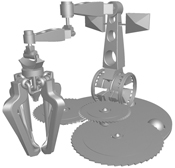
\includegraphics[width=0.5\linewidth]{fig5_15.jpg}
    \caption{Figure 5-15 Per-Vertex Lighting Results}
    \label{fig:5-15}
\end{figure}

\section{5.3 Per-Fragment Lighting}

You may have noticed that the per-vertex lighting results look somewhat coarse. The shading tends to be a bit "triangular" looking, meaning that you can make out the underlying mesh structure, if the model is simple enough. If the model has very few vertices, per-vertex lighting will often be inadequate. However, as your models acquire more and more vertices, you will find that the results start to improve considerably, as in Figure \ref{fig:5-16}. The figure shows three tessellated cylinders with different levels of tessellation. Below each lit cylinder is the wireframe version of the model showing each cylinder's tessellation. As the amount of tessellation increases from left to right, notice that the lighting improves significantly.

\begin{figure}
    \centering
    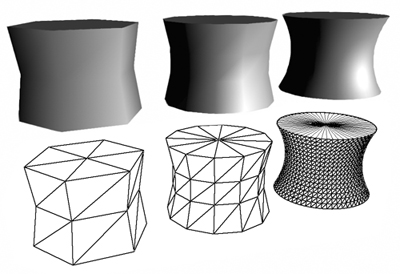
\includegraphics[width=1\linewidth]{fig5_16.jpg}
    \caption{Figure 5-16 The Effects of Tessellation on Lighting}
    \label{fig:5-16}
\end{figure}

Less tessellated models look bad with per-vertex lighting because of the way data is interpolated and used. With per-vertex lighting, lighting is calculated only at each vertex of each triangle. The lighting is then interpolated for each fragment that is generated for the triangle. This approach, called smooth color interpolation or \textit{Gouraud shading}, can miss details because the lighting equation is not actually evaluated for each fragment. For example, a specular highlight that is not captured at any of the triangle's vertices will not show up on the triangle, even if it should appear inside the triangle.

This is exactly what could happen with the preceding per-vertex lighting example: your vertex program calculated the lighting, and then the rasterizer interpolated the colors for each fragment.

To get a more accurate result, you need to evaluate the whole lighting model for each fragment, instead of just for each vertex. So instead of interpolating the final lit color, the surface normals are interpolated. Then, the fragment program uses the interpolated surface normals to calculate the lighting at each pixel. This technique is called \textit{Phong shading} (not to be confused with the Phong lighting model, which refers to the specular approximation used in the Basic model) or, more commonly, \textit{per-pixel lighting} or \textit{per-fragment lighting}. As you might expect, per-fragment lighting gives much better results because the whole lighting equation is evaluated for each fragment of each triangle, as shown in Figure \ref{fig:5-17}. The left side of the figure shows a tessellated cylinder rendered with per-vertex lighting, and the right side shows the same cylinder rendered with per-fragment lighting. Each cylinder has the same coarse tessellation. Notice that the highlights are coarse on the left cylinder and much sharper on the right cylinder.

\begin{figure}
    \centering
    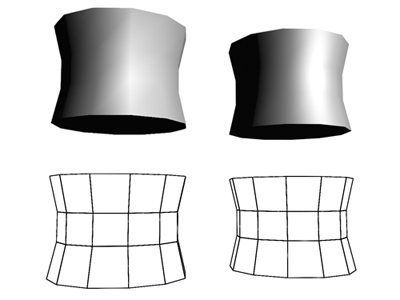
\includegraphics[width=0.75\linewidth]{fig5_17.jpg}
    \caption{Figure 5-17 Comparing Per-Vertex and Per-Fragment Lighting}
    \label{fig:5-17}
\end{figure}

\subsection{5.3.1 Implementing Per-Fragment Lighting}

\begin{framed}
CineFX

The fragment program in this example requires a fourth-generation GPU, such as NVIDIA's GeForce FX or ATI's Radeon 9700.
\end{framed}

In this example, the computational burden on vertex and fragment programs will be swapped; this time, the fragment program will do the interesting work. The vertex program will only help set the stage by passing some parameters over to the fragment program. Many advanced techniques follow this pattern as well, which is probably not very surprising, because fragment programs give you more detailed control over your final image than vertex programs do. Using a vertex or fragment program also has other implications, such as performance. Chapter 10 discusses this topic further.

You will find that the fragment program for per-fragment lighting looks remarkably similar to the vertex program for per-vertex lighting. Again, that is because Cg allows you to use a common language for both vertex and fragment programming. This capability turns out to be very useful for per-fragment lighting, because the required code will already be familiar to you. Like the per-vertex lighting, the per-fragment lighting is done in object space, for ease of implementation.

\subsection{5.3.2 The Vertex Program for Per-Fragment Lighting}

The vertex program for this example is just a conduit: it performs minimal computations and essentially forwards data down the pipeline, so that the fragment program can do the interesting work. After writing out the homogeneous position, the vertex program also passes along the object-space position and object-space normal, outputting them as texture coordinate sets 0 and 1.

Example 5-2 shows the complete source code for the vertex program. There are no new concepts here, so take this opportunity to make sure that you completely understand each line in the program.

\FloatBarrier
\begin{lstlisting}[caption=Example 5-2. The \textbf{C5E2v_fragmentLighting} Vertex Program]
void C5E2v_fragmentLighting(float4 position : POSITION,
                            float3 normal   : NORMAL,

                        out float4 oPosition : POSITION,
                        out float3 objectPos : TEXCOORD0,
                        out float3 oNormal   : TEXCOORD1,

                    uniform float4x4 modelViewProj)
{
  oPosition = mul(modelViewProj, position);
  objectPos = position.xyz;
  oNormal = normal;
}
\end{lstlisting}
\FloatBarrier

\subsection{5.3.3 The Fragment Program for Per-Fragment Lighting}

The \textbf{C5E3f_basicLight} program is almost identical to the vertex program for per-vertex lighting, and so we will not go through it in detail. Example 5-3 shows the source code for the per-fragment lighting program.

It is common to assume that the object-space per-vertex normal is already normalized. In such a case, one operation that \textbf{C5E3f_basicLight} performs that the corresponding vertex program would not require is renormalizing the interpolated per-fragment normal:

\FloatBarrier
\begin{lstlisting}
float3 N = normalize(normal);
\end{lstlisting}
\FloatBarrier

This \textbf{normalize} is necessary because linear interpolation of a texture coordinate set can cause the per-fragment normal vector to become denormalized.

The \textbf{C5E3f_basicLight} fragment program shows that Cg really does allow you to express your ideas the same way in both vertex and fragment programs (as long as your GPU is powerful enough to keep up—this program, as written, requires a fourth-generation GPU or better). But per-fragment calculations aren't free. In most cases, there will be more fragments in the frame than there are vertices, which means that the fragment program needs to run many more times than the vertex program. Therefore, longer fragment programs tend to have a more significant impact on performance than longer vertex programs. Chapter 10 discusses in more detail the trade-offs between using vertex and fragment programs.

\FloatBarrier
\begin{lstlisting}[caption=Example 5-3. The \textbf{C5E3f_basicLight} Fragment Program]
void C5E3f_basicLight(float4 position  : TEXCOORD0,
                      float3 normal    : TEXCOORD1,

                  out float4 color     : COLOR,

              uniform float3 globalAmbient,
              uniform float3 lightColor,
              uniform float3 lightPosition,
              uniform float3 eyePosition,
              uniform float3 Ke,
              uniform float3 Ka,
              uniform float3 Kd,
              uniform float3 Ks,
              uniform float  shininess)
{
  float3 P = position.xyz;
  float3 N = normalize(normal);

  // Compute the emissive term
  float3 emissive = Ke;

  // Compute the ambient term
  float3 ambient = Ka * globalAmbient;

  // Compute the diffuse term
  float3 L = normalize(lightPosition - P);
  float diffuseLight = max(dot(N, L), 0);
  float3 diffuse = Kd * lightColor * diffuseLight;

  // Compute the specular term
  float3 V = normalize(eyePosition - P);
  float3 H = normalize(L + V);
  float specularLight = pow(max(dot(N, H), 0),
                            shininess);
  if (diffuseLight <= 0) specularLight = 0;
  float3 specular = Ks * lightColor * specularLight;

  color.xyz = emissive + ambient + diffuse + specular;
  color.w = 1;
}
\end{lstlisting}
\FloatBarrier

In the rest of this chapter, and the remainder of this book, we avoid complex fragment programs where possible, to make the examples accessible to a broad range of GPU generations. But you can usually move a per-vertex computation to the fragment program if you want to.

\section{5.4 Creating a Lighting Function}

In the preceding section, we simply copied most of the code from the per-vertex example to the per-fragment example, but there's a better solution: encapsulating the key aspects of lighting in a function.

In a complex Cg program, lighting might be only one of several computations that the program performs. In the per-vertex lighting example, you saw the various steps that were necessary to calculate lighting. But you would not want to rewrite all this code whenever you wanted to compute lighting. Fortunately, you don't have to. As we mentioned in Chapter 2, you can write an internal function that encapsulates the lighting task and reuse the same lighting function in different entry functions.

Unlike functions in C or C++, functions in Cg are typically inlined (though this may depend on the profile—advanced profiles such as \textbf{vp30} can support function calls in addition to inlining). Inlining functions means that they have no associated function-call overhead. Therefore, you should use functions whenever possible, because they improve readability, simplify debugging, encourage reuse, and make future optimization easier.

Cg, like C, requires that you declare functions before using them.

\subsection{5.4.1 Declaring a Function}

In Cg, functions are declared just as in C. You can optionally specify parameters to pass to the function, as well as values that will be returned by the function. Here is a simple function declaration:

\FloatBarrier
\begin{lstlisting}
float getX(float3 v)
{
  return v.x;
}
\end{lstlisting}
\FloatBarrier

This function takes a three-component vector \textbf{v} as a parameter and returns a \textbf{float} that is the \textit{x} component of \textbf{v}. The \textbf{return} keyword is used to return the function's result. You call the \textbf{getX} function just as you would call any other Cg function:

\FloatBarrier
\begin{lstlisting}
// Declare a scratch vector
float3 myVector = float3(0.5, 1.0, -1.0);

// Get the x component of myVector
float x = getX(myVector);
// Now x = 0.5
\end{lstlisting}
\FloatBarrier

Sometimes, you want a function to return several results instead of just one. In these situations, you can use the \textbf{out} modifier (as explained in Section 3.3.4) to specify that a particular parameter to a program be for output only. Here is an example that takes a vector and returns its x, y, and z components:

\FloatBarrier
\begin{lstlisting}
void getComponents(float3 vector,
               out float x,
               out float y,
               out float z)
{
  x = vector.x;
  y = vector.y;
  z = vector.z;
}
\end{lstlisting}
\FloatBarrier

Note that this function is declared \textbf{void}, because it returns all its values through parameters. Here is a code sample that shows how \textbf{getComponents} would be used:

\FloatBarrier
\begin{lstlisting}
// Declare a scratch vector
float3 myVector = float3(0.5, 1.0, -1.0);

// Declare scratch variables
float x, y, z;

// Get the x, y, and z components of myVector
getComponents(myVector, x, y, z);
// Now x = 0.5, y = 1.0, z = -1.0
\end{lstlisting}
\FloatBarrier

\subsection{5.4.2 A Lighting Function}

Because lighting is a complex process, you can write many different types of lighting functions, each of which can take different parameters. For now, take the Basic model that you implemented and create a function for it. Here is a first shot at this function:

\FloatBarrier
\begin{lstlisting}
float3 lighting(float3 Ke,
                float3 Ka,
                float3 Kd,
                float3 Ks,
                float  shininess,
                float3 lightPosition,
                float3 lightColor,
                float3 globalAmbient,
                float3 P,
                float3 N,
                float3 eyePosition)
{
  // Calculate lighting here
}
\end{lstlisting}
\FloatBarrier

One major problem with this approach is that the function requires so many parameters. It would be far neater to group the parameters into "material parameters" and "light parameters," and then to pass each set as an individual variable. Fortunately, Cg supports structures, which provide exactly this functionality.

\subsection{5.4.3 Structures}

As we mentioned in Chapter 2, Cg structures are declared the same way they are in C or C++. The \textbf{struct} keyword is used, followed by the list of structure members. Here is an example of a structure that encapsulates all the properties of a particular material based on the Basic lighting model:

\FloatBarrier
\begin{lstlisting}
struct Material {
  float3 Ke;
  float3 Ka;
  float3 Kd;
  float3 Ks;
  float  shininess;
};
\end{lstlisting}
\FloatBarrier

Structure members are accessed using the period operator. The following code snippet shows how to declare and access a structure:

\FloatBarrier
\begin{lstlisting}
Material shiny;
shiny.Ke = float3(0.0, 0.0, 0.0);
shiny.Ka = float3(0.1, 0.1, 0.1);
shiny.Kd = float3(0.2, 0.4, 0.2);
shiny.Ks = float3(0.8, 0.8, 0.8);
shiny.shininess = 90.0;
\end{lstlisting}
\FloatBarrier

You could create a second structure to hold light properties:

\FloatBarrier
\begin{lstlisting}
struct Light {
  float4 position;
  float3 color;
};
\end{lstlisting}
\FloatBarrier

Now, you can redefine the lighting function using structures as parameters:

\FloatBarrier
\begin{lstlisting}
float3 lighting(Material material,
                Light light,
                float3 globalAmbient,
                float3 P,
                float3 N,
                float3 eyePosition)
{
  // Calculate lighting here
}
\end{lstlisting}
\FloatBarrier

With this approach, you could later make your light or material model more complex, without having to add more parameters to the lighting function itself. Another advantage is that you can calculate the effects of multiple lights by using an array of \textbf{Light} structures instead of just one.

\subsection{5.4.4 Arrays}

Cg supports arrays much as C does. Because Cg currently does not support pointers, you must always use array syntax rather than pointer syntax when dealing with arrays. Here is an example of an array declaration and access in Cg:

\FloatBarrier
\begin{lstlisting}
// Declare a four-element array
float3 myArray[4];
int index = 2;

// Assign a vector to element 2 of the array
myArray[index] = float3(0.1, 0.2, 0.3);
\end{lstlisting}
\FloatBarrier

\begin{framed}
Advanced Topic

An important difference from C is that arrays are first-class types in Cg. This means that array assignments actually copy the entire array, and arrays that are passed as parameters are passed by value (the entire array is copied before making any changes), rather than by reference.
\end{framed}

You can also pass arrays as parameters to functions. We're going to use this feature to create a function that computes the lighting from two distinct light sources, as shown in Example 5-4.

As you look over the code for \textbf{C5E4v_twoLights} , you will notice that it starts by calculating the emissive and ambient terms, which are independent of the light sources. The function then loops over the two light sources using a \textbf{for} loop, accumulating the diffuse and specular contributions from the lights. These contributions are calculated using the \textbf{C5E5_computeLighting} helper function, which we will define shortly. First, let's learn a little more about \textbf{for} loops and other constructs that control the flow of Cg programs.

\subsection{5.4.5 Flow Control}

Cg offers a subset of C's flow-control capabilities. In particular, Cg supports:

\begin{enumerate}
\item functions and the \textbf{return} statement
\item \textbf{if}-\textbf{else}
\item \textbf{for}
\item \textbf{while} and \textbf{do}-\textbf{while}
\end{enumerate}

These are identical to their C counterparts, except for profile-specific restrictions that may exist. For example, some profiles allow \textbf{for} or \textbf{while} loops only if the number of loop iterations can be determined ahead of time by the Cg compiler.

Cg reserves keywords for other C flow-control constructs, such as \textbf{goto} and \textbf{switch}. However, these constructs are not currently supported.

\FloatBarrier
\begin{lstlisting}[caption=Example 5-4. The \textbf{C5E4v_twoLights} Vertex Program]
void C5E4v_twoLights(float4 position : POSITION,
                     float3 normal   : NORMAL,

                 out float4 oPosition : POSITION,
                 out float4 color     : COLOR,
             
             uniform float4x4 modelViewProj,
             uniform float3   eyePosition,
             uniform float3   globalAmbient,
             uniform Light    lights[2],
             uniform float    shininess,
             uniform Material material)
{
  oPosition = mul(modelViewProj, position);

  // Calculate emissive and ambient terms
  float3 emissive = material.Ke;
  float3 ambient = material.Ka * globalAmbient;

  // Loop over diffuse and specular contributions
  // for each light
  float3 diffuseLight;
  float3 specularLight;
  float3 diffuseSum   = 0;
  float3 specularSum  = 0;
  for (int i = 0; i < 2; i++) {
    C5E5_computeLighting(lights[i], position.xyz, normal,
                         eyePosition, shininess, diffuseLight,
                         specularLight);
    diffuseSum += diffuseLight;
    specularSum += specularLight;
  }

  // Now modulate diffuse and specular by material color
  float3 diffuse = material.Kd * diffuseSum;
  float3 specular = material.Ks * specularSum;

  color.xyz = emissive + ambient + diffuse + specular;
  color.w = 1;
}
\end{lstlisting}
\FloatBarrier

\subsection{5.4.6 Computing the Diffuse and Specular Lighting}

The final piece of the puzzle is the \textbf{C5E5_computeLighting} function, which is responsible for calculating the diffuse and specular contributions for a particular light source. Example 5-5 re-implements the diffuse and specular lighting code that we wrote earlier.

\FloatBarrier
\begin{lstlisting}[caption=Example 5-5. The C5E5_computeLighting Internal Function]
void C5E5_computeLighting(Light  light,
                          float3 P,
                          float3 N,
                          float3 eyePosition,
                          float  shininess,

                      out float3 diffuseResult,
                      out float3 specularResult)
{
  // Compute the diffuse lighting
  float3 L = normalize(light.position - P);
  float diffuseLight = max(dot(N, L), 0);
  diffuseResult = light.color * diffuseLight;

  // Compute the specular lighting
  float3 V = normalize(eyePosition - P);
  float3 H = normalize(L + V);
  float specularLight = pow(max(dot(N, H), 0),
                            shininess);
  if (diffuseLight <= 0) specularLight = 0;
  specularResult = light.color * specularLight;
}
\end{lstlisting}
\FloatBarrier

\section{5.5 Extending the Basic Model}

Now that you have implemented a Basic lighting model, let's look at how we can make it a little more useful. The following sections present three enhancements: distance attenuation, spotlight effects, and directional lights. Each enhancement will work at both the vertex level and the fragment level.

Lighting is a very complicated topic, and there are a huge number of techniques to explore. Our goal is just to get you started.

\subsection{5.5.1 Distance Attenuation}

The Basic lighting model assumes that the intensity of the light source is always the same no matter how far the light is from the surface being shaded. Although that is a reasonable approximation for some light sources (such as when the Sun lights objects on Earth), we usually want to create lights for which intensity diminishes with distance. This property is called \textit{distance attenuation}. In OpenGL or Direct3D, the attenuation at any particular point is modeled using the following formula:

$attenuationFactor = \frac{1}{k_c + k_Ld + k_Qd^2}$

where:

\begin{itemize}
\item $d$ is the distance from the light source and
\item $k_C$, $k_L$, and $k_Q$ are constants that control the amount of attenuation.
\end{itemize}

In this formulation of attenuation, $k_C$, $k_L$, and $k_Q$, respectively, are the constant, linear, and quadratic coefficients of attenuation. In the real world, the intensity of illumination from a point light source decays as $1/d^2$, but sometimes that might not give the effect you want. The idea behind having three attenuation parameters is to give you more control over the appearance of your scene's lighting.

The attenuation factor modulates the diffuse and specular terms of the lighting equation. So the equation becomes:

$lighting = emissive + ambient + attenuationFactor * (diffuse + specular)$

Example 5-6 describes a Cg function that calculates attenuation, given the surface position and \textbf{Light} structure (to which we have now added \textbf{kC}, \textbf{kL}, and \textbf{kQ}).

\FloatBarrier
\begin{lstlisting}[caption=Example 5-6. The \textbf{C5E6_attenuation} Internal Function]
float C5E6_attenuation(float3 P,
                       Light  light)
{
  float d = distance(P, light.position);
  return 1 / (light.kC + light.kL * d +
              light.kQ * d * d);
}
\end{lstlisting}
\FloatBarrier

We take advantage of the \textbf{distance} function that is yet another one of Cg's Standard Library functions. Here is the formal definition of \textbf{distance}:

\FloatBarrier
\begin{table}
\centering
\begin{tabular}{ p{5cm} p{7cm}  } 
\hline
\textbf{distance(pt1, pt2)} & Euclidean distance between points \textbf{pt1} and \textbf{pt2} \\
\hline
\end{tabular}
\end{table}
\FloatBarrier

The attenuation calculation needs to be added to the \textbf{C5E5_computeLighting} function, because it affects both the diffuse contribution and the specular contribution from the light source. You should calculate the attenuation first, so that you can use it to modulate the diffuse and specular contributions. The \textbf{C5E7_attenuateLighting} internal function in Example 5-7 shows the necessary modifications.

\FloatBarrier
\begin{lstlisting}[caption=Example 5-7. The C5E7_attenuateLighting Internal Function]
void C5E7_attenuateLighting(Light  light,
                            float3 P,
                            float3 N,
                            float3 eyePosition,
                            float  shininess,

                        out float diffuseResult,
                        out float specularResult)
{
  // Compute attenuation
  float attenuation = C5E6_attenuation(P, light);

  // Compute the diffuse lighting
  float3 L = normalize(light.position - P);
  float diffuseLight = max(dot(N, L), 0);
  diffuseResult = attenuation *
                  light.color * diffuseLight;

  // Compute the specular lighting
  float3 V = normalize(eyePosition - P);
  float3 H = normalize(L + V);
  float specularLight = pow(max(dot(N, H), 0),
                            shininess);
  if (diffuseLight <= 0) specularLight = 0;
  specularResult = attenuation *
                   light.color * specularLight;
}
\end{lstlisting}
\FloatBarrier

\subsection{5.5.2 Adding a Spotlight Effect}

Another commonly used extension for the Basic lighting model is making the light a spotlight instead of an omnidirectional light. A spotlight cut-off angle controls the spread of the spotlight cone, as shown in Figure \ref{fig:5-18}. Only objects within the spotlight cone receive light.

\begin{figure}
    \centering
    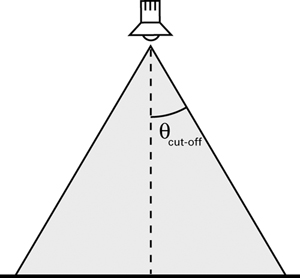
\includegraphics[width=0.5\linewidth]{fig5_18.jpg}
    \caption{Figure 5-18 Specifying a Spotlight Cut-Off Angle}
    \label{fig:5-18}
\end{figure}

To create the spotlight cone, you need to know the spotlight position, spotlight direction, and position of the point that you are trying to shade. With this information, you can compute the vectors \textit{V} (the vector from the spotlight to the vertex) and \textit{D} (the direction of the spotlight), as shown in Figure \ref{fig:5-19}.

\begin{figure}
    \centering
    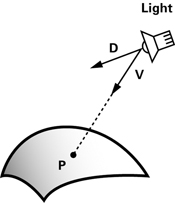
\includegraphics[width=0.5\linewidth]{fig5_19.jpg}
    \caption{Figure 5-19 Vectors for Calculating the Spotlight Effect}
    \label{fig:5-19}
\end{figure}

By taking the dot product of the two normalized vectors, you can find the cosine of the angle between them, and use that to find out if \textit{P} lies within the spotlight cone. \textit{P} is affected by the spotlight only if \textbf{dot(V, D)} is greater than the cosine of the spotlight's cut-off angle.

Based on this math, we can create a function for the spotlight calculation, as shown in Example 5-8. The function \textbf{C5E8_spotlight} returns 1 if \textit{P} is within the spotlight cone, and 0 otherwise. Note that we have added \textbf{direction} (the spotlight direction—assumed to be normalized already) and \textbf{cosLightAngle} (the cosine of the spotlight's cut-off angle) to the \textbf{Light} structure from Example 5-6.

\FloatBarrier
\begin{lstlisting}[caption=Example 5-8. The \textbf{C5E8_spotlight} Internal Function]
float C5E8_spotlight(float3 P,
                     Light  light)
{
  float3 V = normalize(P - light.position);
  float cosCone = light.cosLightAngle;
  float cosDirection = dot(V, light.direction);
  if (cosCone <= cosDirection)
    return 1;
  else
    
   return 0;
}
\end{lstlisting}
\FloatBarrier

\subsection*{Intensity Variation}

So far, we have assumed that the intensity of light given off by the spotlight is uniform within the spotlight's cone. Rarely, if ever, is a real spotlight so uniformly focused. To make things more interesting, we will divide the cone into two parts: an inner cone and an outer cone. The inner cone (or "hotspot") emits a constant intensity, and this intensity drops off smoothly outside the cone, as shown in Figure \ref{fig:5-20}. This commonly used approach creates the more sophisticated effect demonstrated in the right side of Figure \ref{fig:5-21}.

\begin{figure}
    \centering
    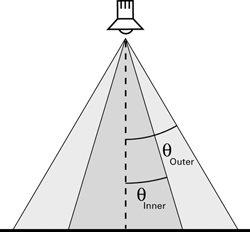
\includegraphics[width=0.5\linewidth]{fig5_20.jpg}
    \caption{Figure 5-20 Specifying Inner and Outer Cones for a Spotlight}
    \label{fig:5-20}
\end{figure}

\begin{figure}
    \centering
    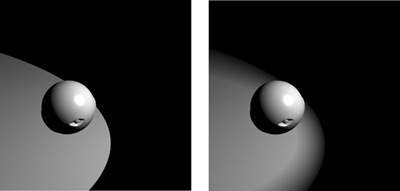
\includegraphics[width=1\linewidth]{fig5_21.jpg}
    \caption{Figure 5-21 The Effect of Adding Inner and Outer Spotlight Cones}
    \label{fig:5-21}
\end{figure}

It's not hard to find out if a particular point \textit{P} is in the inner cone or the outer cone. The only difference from the basic spotlight is that you now need to vary the intensity calculation based on which cone \textit{P} lies.

If \textit{P} lies in the inner cone, it receives the spotlight's full intensity. If \textit{P} lies in between the inner and outer cones, you need to lower the intensity gradually based on how far \textit{P} is from the inner cone. Cg's \textbf{lerp} function works well for this type of transition, but with advanced profiles, you can do better.

Cg has a \textbf{smoothstep} function that produces more visually appealing results than a simple \textbf{lerp}. Unfortunately, the \textbf{smoothstep} function might not work with some basic profiles, because of their limited capabilities. We'll use \textbf{smoothstep} in this example, though you could replace it with another function of your choice.

The \textbf{smoothstep} function interpolates between two values, using a smooth polynomial:

\FloatBarrier
\begin{table}
\centering
\begin{tabular}{ p{5cm} p{7cm}  } 
\hline

\textbf{smoothstep(min, max, x)} & Returns \textbf{0} if \verb!x < min!; \\
& Returns \textbf{1} if \verb!x >= max!; \\
& Otherwise, returns a smooth Hermite \\
& interpolation between 0 and 1 given by: \\
& \textbf{-2 * ((x – min)/(max – min))\textsuperscript{3} +} \\
& \textbf{3 * ((x – min)/(max – min))\textsuperscript{2}} \\
\hline
\end{tabular}
\end{table}
\FloatBarrier

Figure \ref{fig:5-22} graphs what the \textbf{smoothstep} function looks like. Use \textbf{smoothstep} when you want to create a visually pleasing transition between two values. Another convenient feature of \textbf{smoothstep} is that it clamps to the [0, 1] range. If you set up your parameters to \textbf{smoothstep} correctly, it will return 1.0 when \textit{P} is in the inner cone, and 0.0 when \textit{P} is outside the outer cone.

\begin{figure}
    \centering
    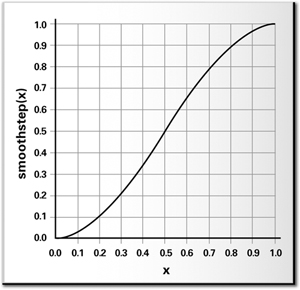
\includegraphics[width=0.5\linewidth]{fig5_22.jpg}
    \caption{Figure 5-22 A Graph of the Function}
    \label{fig:5-22}
\end{figure}

Once again, we can extend the \textbf{Light} structure to include the new spotlight parameters. The single cut-off angle is now replaced by an inner angle cosine and an outer angle cosine.

Here is how our further updated version of the \textbf{Light} structure looks:

\FloatBarrier
\begin{lstlisting}
struct Light {
  float4 position;
  float3 color;
  float  kC;
  float  kL;
  float  kQ;
  float3  direction;
  float  cosInnerCone; // New member
  float  cosOuterCone; // New member
};
\end{lstlisting}
\FloatBarrier

The \textbf{C5E9_dualConeSpotlight} internal function shown in Example 5-9 combines all this to create a spotlight with a hotspot.

The \textbf{C5E10_spotAttenLighting} internal function combines both the attenuation and the spotlight terms with specular and diffuse lighting, as shown in Example 5-10.

\FloatBarrier
\begin{lstlisting}[caption=Example 5-9. The \textbf{C5E9_dualConeSpotlight} Internal Function]
float C5E9_dualConeSpotlight(float3 P,
                             Light  light)
{
  float3 V = normalize(P - light.position);
  float cosOuterCone = light.cosOuterCone;
  float cosInnerCone = light.cosInnerCone;
  float cosDirection = dot(V, light.direction);
  return smoothstep(cosOuterCone,
                    cosInnerCone,
                    cosDirection);
}
\end{lstlisting}
\FloatBarrier

\FloatBarrier
\begin{lstlisting}[caption=Example 5-10. The \textbf{C5E10_spotAttenLighting} Internal Function]
void C5E10_spotAttenLighting(Light  light,
                             float3 P,
                             float3 N,
                             float3 eyePosition,
                             float  shininess,

                         out float diffuseResult,
                         out float specularResult)
{
  // Compute attenuation
  float attenuationFactor = C5E6_attenuation(P, light);

  // Compute spotlight effect
  float spotEffect = C5E9_dualConeSpotlight(P, light);

  // Compute the diffuse lighting
  float3 L = normalize(light.position - P);
  float diffuseLight = max(dot(N, L), 0);
  diffuseResult = attenuationFactor * spotEffect *
                  light.color * diffuseLight;

  // Compute the specular lighting
  float3 V = normalize(eyePosition - P);
  float3 H = normalize(L + V);
  float specularLight = pow(max(dot(N, H), 0),
                            shininess);
  if (diffuseLight <= 0) specularLight = 0;
  specularResult = attenuationFactor * spotEffect *
                   light.color * specularLight;
}
\end{lstlisting}
\FloatBarrier

\subsection{5.5.3 Directional Lights}

Although computations such as the spotlight effect and attenuation add to the visual complexity of your scenes, the results are not always noticeable. Consider rays from the Sun that light objects on Earth. All the rays seem to come from the same direction because the Sun is so far away. In such a situation, it does not make sense to calculate a spotlight effect or to add attenuation, because all objects receive essentially the same amount of light. A light with this property is called a \textit{directional light}. Directional lights do not exist in reality, but in computer graphics, it is often worthwhile to identify situations in which a directional light is sufficient. This allows you to avoid computations that will not produce perceptible results.

\section{5.6 Exercises}

\begin{enumerate}

\item \textbf{Answer this:} What visual differences distinguish surfaces rendered with a per-vertex lighting model from those rendered with a per-fragment lighting model? In particular, discuss specular highlights and spotlights.

\item \textbf{Try this yourself:} Modify the \textbf{C5E5_computeLighting} function to assume a directional light, as described in Section 5.5.3. You should be able to improve the function's performance by eliminating a vector difference and through normalization.

\item \textbf{Try this yourself:} The lighting examples in this chapter assume that your application specifies the light position in object space. You could also specify light positions in eye space. Using eye space to specify light positions is convenient because it avoids requiring the application to transform the light position from world or eye space into object space for each object's distinct object space. Also, the view vector for computing the specular contribution is simply the eye-space vertex position because the eye is at the origin. Lighting in eye space, however, requires transforming the object-space position and normal into eye space for every vertex. Transforming an object-space position and normal into eye space requires multiplying each by the modelview matrix and inverse transpose of the modelview matrix, respectively. If the modelview matrix scales vectors, you must normalize the eye-space normal, because the modelview matrix would denormalize the normal. Modify the \textbf{C5E5_computeLighting} function to assume that the position \textbf{P} and normal \textbf{N} are in eye space. Also, modify \textbf{C5E4v_twoLights} to transform the object-space position and normal into eye space prior to passing these vectors to your new \textbf{C5E5_computeLighting} function.

\item \textbf{Try this yourself:} Modify the eye-space version of the \textbf{C5E5_computeLighting} function you implemented for Exercise 3 to assume that the eye-space vector \textbf{V} is always in the direction (0, 0, 1). This is known as the \textit{infinite viewer} specular optimization, and it eliminates the requirement to normalize \textbf{V} prior to computing \textbf{H}. How much does this change your rendering results? Is this optimization possible when implementing object-space lighting?

\item \textbf{Answer this:} Which is more efficient: object-space or eye-space lighting? Also, which is more convenient for the application programmer?

\item \textbf{Try this yourself:} Write a pair of Cg vertex and fragment programs that mix per-vertex and per-fragment lighting. Compute the emissive, ambient, and diffuse contributions in the vertex program. Also, compute the half-angle and normal vectors in the vertex program, and then pass these vectors to your fragment program. In the fragment program, compute just the specular contribution using the interpolated half-angle and normal vectors. This partitioning of the lighting task means that most of the lighting math occurs at the per-vertex level, but the specular contribution that is the most subject to per-vertex artifacts is computed at the per-fragment level for better quality. Compare the quality and performance of this approach to a pure per-vertex and per-fragment lighting implementation.

\item \textbf{Try this yourself:} Brushed or grooved surfaces such as hair, vinyl records, satin Christmas ornaments, and brushed metal finishes reflect light differently than conventional materials do because the grooved microstructure of these surfaces creates anisotropic light scattering. Research the topic of anisotropic lighting as discussed in the "Further Reading" section. Create a vertex or fragment program that implements anisotropic lighting.

\end{enumerate}

\section{5.7 Further Reading}

The lighting chapter of the \textit{OpenGL Programming Guide: The Official Guide to Learning OpenGL, Third Edition} (Addison-Wesley, 1999), by Mason Woo, Jackie Neider, Tom Davis, and Dave Shreiner, presents the complete OpenGL fixed-function lighting model. Although the presentation is OpenGL-centric, the corresponding Direct3D fixed-function lighting model is almost identical. To find out more about Direct3D's lighting model, refer to "Mathematics of Lighting" in Microsoft's online DirectX documentation.

Eric Lengyel's book \textit{Mathematics for 3D Game Programming and Computer Graphics} (Charles River Media, 2001) has a good chapter titled "Illumination" that discusses the practical math for implementing various lighting models.

David Banks published a SIGGRAPH paper titled "Illumination in Diverse Codimensions" (ACM Press) in 1994 that discussed anisotropic lighting. Wolfgang Heidrich and Hans-Peter Seidel published "Efficient Rendering of Anisotropic Surfaces Using Computer Graphics Hardware" in 1998; that paper, which applied anisotropic lighting to a surface in real time, provides the equations you will need for Exercise 7.

Robert Cook and Kenneth Torrance published a detailed, physically plausible lighting model in a paper titled "A Reflectance Model for Computer Graphics" in \textit{ACM Transactions on Graphics} in 1982.

Andrew Glassner's two-volume \textit{Principles of Digital Image Synthesis} (Morgan Kaufmann, 1995) is a detailed study of how light interacts with materials, approached from a computer graphics viewpoint.

\end{document}